Dialog System Technology Challenges 8 \cite{dstc8}とは対話に関するコンペティションである.2013 年に最初の Dialog State Tracking Challenge(対話状態追跡タスク)が開催された.第 6 回から対話状態追跡だけでなく,対話破綻検出や応答生成といった対象となるタスクの幅が広がり,略称はDSTCのままで現在の Dialog System Technology Challenges へと名称が変更された.\par
第 8 回 DSTC にあたる Dialog System Technology Challenges 8 では,End-to-Endのニューラルネットワークを用いた対話システムを作成する Dialogue System トラック,対話履歴に対して多数の応答候補文から正解となる応答文を選択する Sentence Selection トラック,画像とそれに関する質問に応じた応答を生成する Audio Visual Scene-aware dialog トラック,学習していないドメインにも対応可能な対話状態追跡を行う Dialogue State Tracking の4つのトラックが存在する.\par
ここでは本研究で取り組んだ Dialogue State Tracking トラック について説明する.DSTC8-Track4は,Google Assistantなど現在のタスク指向型対話システムの課題の1つである新サービスへの拡張を可能にすることを目的としたトラックである.本トラックの最大の特徴として,訓練時,検証時,テスト時それぞれで扱うサービスの一部が異なることが挙げられる.具体的には図\ref{fig:dstc8-track4}に示した通り,同じ Flight Service でもユーザの目標であるインテントの候補とユーザの要求を表すスロットが異なる名前で定義されている.そして,どちらのサービスを扱うとしても,ユーザの目標と要求を正しく推定できる対話状態追跡モデルを作成することが本トラックの目的である.また,このインテントとスロットを定義する枠組みをスキーマと呼ぶ.\par 
\begin{figure}[tbh]
    \centering
    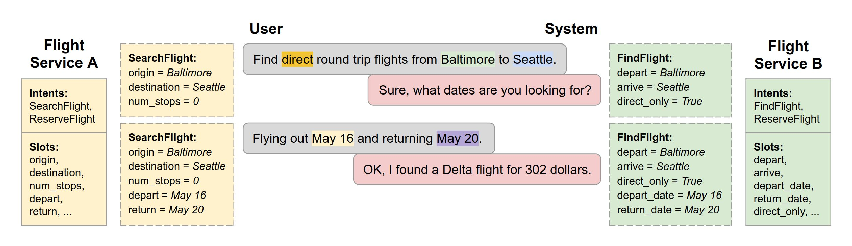
\includegraphics[width=15cm]{chapter2/dstc8-track4.eps}
    \caption{DSTC8-Track4 のイメージ図}
    \label{fig:dstc8-track4}
\end{figure}
参加者はベースラインモデルと整形された対話データセットが配布され,そのデータセットなどを用いて作成したモデルの訓練と評価を行い,モデルと評価結果を提出する.ただし,本研究では配布されたベースラインモデルと対話データセットを利用しただけであり,DSTC8-Track4 には提出していない.\par 
配布されたデータセットは人と機械の間の 18K 以上の注釈付きマルチドメインタスク指向の対話で,各対話は以下のような構成である.
\begin{itemize}
    \item 対話ID - 各対話に与えられる識別子
    \item サービスリスト - 対話中に扱うサービスのリスト
    \item ターンリスト - 注釈付きのユーザあるいはシステム発話のリスト
\end{itemize}
また,各ターンは以下の要素を持つ
\begin{itemize}
    \item スピーカー - 発話者がユーザかシステムか
    \item 発話文 - 自然言語発話
    \item フレームリスト - 注釈の内容を表すフレームのリスト
\end{itemize}
続いて,各フレームの要素を示す.フレームは扱うサービスごとに1つ与えられる.
\begin{itemize}
    \item サービス - フレームに対応するサービスの名前
    \item スロット値候補リスト - 発話中に存在するスロット値候補のリスト
    \begin{itemize}
        \item[〇] スロット - スロットの名前
        \item[〇] 開始位置 - 発話中にあるスロット値候補の文字列の開始位置
        \item[〇] 終了位置 - 発話中にあるスロット値候補の文字列の終了位置
    \end{itemize}
    \item 対話行為リスト(システムのターンのみ) - システムがその発話で行った行為のリスト
    \item 対話状態(ユーザのターンのみ) - サービスに対応する対話状態
    \begin{itemize}
        \item[〇] インテント - サービスに対応する現在のユーザの目標(Noneを含む)
        \item[〇] 要求スロット - ユーザがスロット値を要求しているスロットのリスト
        \item[〇] スロット値 - 各スロットに当てはまる値を対応付けた辞書
    \end{itemize}
\end{itemize}
\par
本トラックで推定しなければならないものは,対話状態に含まれる,インテント,要求スロット,スロット値の3つである.また,スロット値候補リストもテストデータでは与えられないので,任意で推定を行うことが可能である.